% Gabarit pandoc des corrigés publiés (brut et guidé). Contenu sans marque ni nom de site.
% Compilation : lualatex (latexmk -lualatex).
% Le Markdown reste la source unique : ne pas éditer ce fichier .tex à la main.
\documentclass[11pt,a4paper]{article}

% --- Moteur, polices (Latin Modern) et langue ---------------------------------
\usepackage{iftex}
\ifLuaTeX\else\errmessage{Ce document se compile avec lualatex}\fi
\usepackage{amsmath,amssymb,mathtools}
\usepackage{fontspec}
% mathrm=sym : \mathrm prend ses glyphes dans la police mathématique (ℓ, μ, Ω), comme KaTeX.
\usepackage[math-style=TeX,bold-style=TeX,mathrm=sym]{unicode-math}
% Repli pour les glyphes absents de Latin Modern (indices et exposants Unicode,
% flèches, filets des schémas en texte, symboles) : DejaVu, puis Latin Modern Math
% (ℓ, lettres mathématiques Unicode des légendes).
\directlua{
  luaotfload.add_fallback("repliTexte", {"DejaVuSerif:mode=harf;", "DejaVuSans:mode=harf;", "file:latinmodern-math.otf:mode=harf;"})
  luaotfload.add_fallback("repliMono", {"DejaVuSansMono:mode=harf;", "DejaVuSans:mode=harf;", "file:latinmodern-math.otf:mode=harf;"})
}
\setmainfont{Latin Modern Roman}[RawFeature={fallback=repliTexte}]
\setsansfont{Latin Modern Sans}[RawFeature={fallback=repliTexte}]
\setmonofont{Latin Modern Mono}[RawFeature={fallback=repliMono}]
\setmathfont{Latin Modern Math}
\usepackage[french]{babel}
\frenchsetup{SmallCapsFigTabCaptions=false}

% --- Mise en page --------------------------------------------------------------
\usepackage[a4paper,margin=2.2cm,headheight=14pt,footskip=1.2cm]{geometry}
\usepackage{microtype}
\setlength{\emergencystretch}{4em}
\tolerance=1500
\setlength{\parindent}{0pt}
\setlength{\parskip}{0.55\baselineskip plus 2pt minus 1pt}
\usepackage{xcolor}
% Gris nommés : babel-french rend « ! » actif dans le document.
\definecolor{gris2}{gray}{0.98}
\definecolor{gris3}{gray}{0.97}
\definecolor{gris5}{gray}{0.95}
\definecolor{gris35}{gray}{0.65}
\definecolor{gris40}{gray}{0.60}
\definecolor{gris45}{gray}{0.55}
\definecolor{gris50}{gray}{0.50}
\definecolor{gris55}{gray}{0.45}
\definecolor{gris60}{gray}{0.40}
\definecolor{gris65}{gray}{0.35}
\definecolor{gris70}{gray}{0.30}
\definecolor{gris80}{gray}{0.20}
\definecolor{gris85}{gray}{0.15}
\usepackage{graphicx}
\usepackage{float}
\usepackage{caption}
\captionsetup{font=small,labelformat=empty,justification=centering}
\usepackage{booktabs,longtable,array,multirow,calc}
\usepackage{siunitx}
\sisetup{locale=FR}
\usepackage[version=4]{mhchem}
\usepackage{listings}
\usepackage{fancyhdr}
\usepackage{lastpage}
\usepackage[most]{tcolorbox}
\usepackage{enumitem}
\setlist{nosep,leftmargin=*,topsep=2pt}
\usepackage[hidelinks,unicode]{hyperref}
\usepackage{bookmark}
\hypersetup{pdftitle={Centrale-Supélec PC — Mathématiques 1 2026},pdfauthor={Rédigé par IA},pdfcreator={LaTeX},pdfsubject={Corrigé brut}}
\usepackage{xurl}

% --- Pandoc : listes, tableaux, figures ----------------------------------------
\providecommand{\passthrough}[1]{#1}
\providecommand{\tightlist}{\setlength{\itemsep}{0pt}\setlength{\parskip}{0pt}}

\makeatletter
\def\maxwidth{\ifdim\Gin@nat@width>\linewidth\linewidth\else\Gin@nat@width\fi}
\def\maxheight{\ifdim\Gin@nat@height>0.55\textheight 0.55\textheight\else\Gin@nat@height\fi}
\makeatother
\setkeys{Gin}{width=\maxwidth,height=\maxheight,keepaspectratio}
\setcounter{secnumdepth}{-\maxdimen}
\providecommand{\pandocbounded}[1]{#1}
\usepackage{longtable,booktabs,array}

% --- Code (listings) -----------------------------------------------------------
\lstset{
  basicstyle=\ttfamily\small,
  columns=fullflexible,
  keepspaces=true,
  breaklines=true,
  breakatwhitespace=false,
  postbreak=\mbox{\textcolor{gris50}{$\hookrightarrow$}\space},
  frame=single,
  rulecolor=\color{gris35},
  framesep=4pt,
  xleftmargin=5pt,xrightmargin=5pt,
  backgroundcolor=\color{gris3},
  keywordstyle=\bfseries,
  commentstyle=\color{gris65},
  stringstyle=\color{gris80},
  showstringspaces=false,
  tabsize=4,
  extendedchars=true,
  aboveskip=6pt,belowskip=6pt,
}

% --- Macros des corrigés (KaTeX ↔ LaTeX) ---------------------------------------
% Les corrigés sont écrits pour KaTeX : on définit ici ce que KaTeX connaît et
% que LaTeX n'a pas, sans jamais retoucher le Markdown.
\providecommand{\R}{\mathbb{R}}
\providecommand{\N}{\mathbb{N}}
\providecommand{\Z}{\mathbb{Z}}
\providecommand{\Q}{\mathbb{Q}}
\providecommand{\C}{\mathbb{C}}
\providecommand{\dd}{\mathrm{d}}
\providecommand{\llbracket}{\lBrack}
\providecommand{\rrbracket}{\rBrack}
\providecommand{\lBrace}{\lbrace}
\providecommand{\rBrace}{\rbrace}
\providecommand{\Box}{\square}
\providecommand{\Diamond}{\lozenge}
\providecommand{\varnothing}{\emptyset}
\providecommand{\argmax}{\operatorname*{arg\,max}}
\providecommand{\argmin}{\operatorname*{arg\,min}}
\renewcommand{\leq}{\leqslant}
\renewcommand{\geq}{\geqslant}

% Équation hors texte : réduite à la largeur de la ligne si elle déborde.
\newsavebox{\boiteequation}
\newcommand{\equationajustee}[1]{%
  \sbox{\boiteequation}{$\displaystyle #1$}%
  \ifdim\wd\boiteequation>\linewidth
    \[\resizebox{\linewidth}{!}{\usebox{\boiteequation}}\]%
  \else
    \[#1\]%
  \fi}

% --- Encadrés pédagogiques (sobres, lisibles en noir et blanc) -----------------
\tcbset{
  encadre/.style={
    enhanced,breakable,sharp corners,
    colback=white,colframe=gris55,
    boxrule=0.4pt,leftrule=2.2pt,
    left=6pt,right=6pt,top=3pt,bottom=3pt,
    before skip=6pt,after skip=6pt,
    fonttitle=\bfseries\small,coltitle=black,
    attach title to upper,after title={\quad},
    parbox=false,
  }
}
\newtcolorbox{indication}[1]{encadre,colframe=gris45,colback=gris2,title={Indication~#1}}
\newtcolorbox{methode}{encadre,colframe=gris70,title={Méthode}}
\newtcolorbox{piege}{encadre,colframe=gris85,boxrule=0.8pt,leftrule=2.2pt,title={Piège}}
\newtcolorbox{jury}{encadre,colframe=gris60,colback=gris5,title={Jury}}
\newtcolorbox{encadrenote}{encadre,colframe=gris40}

% --- Titres de section ---------------------------------------------------------
\usepackage{titlesec}
\titleformat{\section}{\Large\bfseries}{}{0pt}{}
\titleformat{\subsection}{\large\bfseries}{}{0pt}{}
\titleformat{\subsubsection}{\normalsize\bfseries}{}{0pt}{}
\titlespacing*{\section}{0pt}{14pt plus 4pt minus 2pt}{6pt}
\titlespacing*{\subsection}{0pt}{10pt plus 3pt minus 2pt}{4pt}
\titlespacing*{\subsubsection}{0pt}{8pt plus 2pt minus 2pt}{2pt}

% --- En-tête et pied de page ---------------------------------------------------
\pagestyle{fancy}
\fancyhf{}
\fancyhead[L]{\small\textsc{Corrigé brut} · Centrale-Supélec PC}
\fancyhead[R]{\small Maths 1 2026}
\fancyfoot[L]{\footnotesize Corrigé rédigé par IA, non officiel}
\fancyfoot[R]{\footnotesize \thepage\,/\,\pageref*{LastPage}}
\renewcommand{\headrulewidth}{0.4pt}
\renewcommand{\footrulewidth}{0pt}
\fancypagestyle{plain}{\fancyhf{}\fancyfoot[R]{\footnotesize \thepage\,/\,\pageref*{LastPage}}\fancyfoot[L]{\footnotesize Corrigé rédigé par IA, non officiel}\renewcommand{\headrulewidth}{0pt}}

\begin{document}
\thispagestyle{plain}
\begin{center}
  {\small\scshape Corrigé brut}\par\smallskip
  {\LARGE\bfseries Centrale-Supélec PC — Mathématiques 1 2026\par}\medskip
  {\large Centrale-Supélec · PC · Maths 1 · 2026\par}
\end{center}
\vspace{2pt}\hrule\vspace{8pt}

\emph{Corrigé rédigé par IA, non officiel. Signalez toute erreur.}

\textbf{Découverte de la planète Neptune} --- 4 heures, calculatrice autorisée. Quatre parties indépendantes, 34 questions.

Convention : le polynôme caractéristique est \(P_A=\det(XI_3-A)\), unitaire (c'est celle du programme, et l'énoncé l'utilise puisqu'il annonce en Q21 que \(P_A\) est le polynôme unitaire \(R\)).

\begin{center}\rule{0.5\linewidth}{0.5pt}\end{center}

\hypertarget{partie-a-uxe9tude-du-mouvement-dune-planuxe8te-seulement-soumise-uxe0-lattraction-du-soleil}{%
\section{Partie A --- Étude du mouvement d'une planète seulement soumise à l'attraction du soleil}\label{partie-a-uxe9tude-du-mouvement-dune-planuxe8te-seulement-soumise-uxe0-lattraction-du-soleil}}

On rappelle les données : \(0<c<a\) et \(b=\sqrt{a^2-c^2}>0\).
Les foyers sont \(F=(c,0)\) et \(F'=(-c,0)\), donc \(FF'=2c\).
Enfin \(\mathcal{E}=\{M\in P : MF+MF'=2a\}\).

\hypertarget{i-uxe9quation-ruxe9duite-de-mathcale}{%
\subsection{\texorpdfstring{I --- Équation réduite de \(\mathcal{E}\)}{I --- Équation réduite de \textbackslash mathcal\{E\}}}\label{i-uxe9quation-ruxe9duite-de-mathcale}}

\textbf{Q1.} L'inégalité triangulaire appliquée aux points \(M,F,F'\) donne \(FF'\leqslant MF+MF'\). Plus généralement, chaque distance est majorée par la somme des deux autres. Ainsi
\equationajustee{\begin{aligned}
MF&\leqslant MF'+F'F,\\
MF'&\leqslant MF+FF'.
\end{aligned}}
On en tire \(MF-MF'\leqslant FF'\) et \(MF'-MF\leqslant FF'\).
Comme \(|MF-MF'|\) est l'un des deux nombres \(MF-MF'\) ou \(MF'-MF\),
\equationajustee{\boxed{FF'\geqslant |MF-MF'|.}}

\textbf{Q2.} Par Q1 et \(c<a\), on a \(|MF-MF'|\leqslant FF'=2c<2a\).
D'une part \(MF-MF'\leqslant 2c<2a\), soit \(MF-MF'-2a<0\).
D'autre part \(MF-MF'\geqslant -2c>-2a\), soit \(MF-MF'+2a>0\). En particulier
\equationajustee{\boxed{\begin{aligned}
MF-MF'-2a&\neq 0,\\
MF-MF'+2a&\neq 0.
\end{aligned}}}

\textbf{Q3.} Notons \(\Pi\) le produit des quatre facteurs. On a \(MF'+MF+2a\geqslant 2a>0\), et les deux derniers facteurs sont non nuls par Q2.
Le produit de ces trois facteurs est donc non nul. Ainsi \(\Pi=0\) si et seulement si \(MF'+MF-2a=0\), c'est-à-dire si et seulement si \(M\in\mathcal{E}\) :
\equationajustee{\boxed{M\in\mathcal{E}\iff (MF'+MF-2a)(MF'+MF+2a)(MF-MF'-2a)(MF-MF'+2a)=0.}}

\textbf{Q4.} On groupe les facteurs conjugués :
\equationajustee{\Pi=\big[(MF+MF')^2-4a^2\big]\big[(MF-MF')^2-4a^2\big].}
Posons \(s=(MF)^2+(MF')^2-4a^2\) et \(p=2\,MF\cdot MF'\). Alors
\equationajustee{\begin{aligned}
(MF+MF')^2-4a^2&=s+p,\\
(MF-MF')^2-4a^2&=s-p,
\end{aligned}}
donc \(\Pi=s^2-p^2\). Par Q3 :
\equationajustee{\boxed{M\in\mathcal{E}\iff \big((MF')^2+(MF)^2-4a^2\big)^2=4(MF')^2(MF)^2.}}

\textbf{Q5.} On a \((MF)^2=(x-c)^2+y^2\) et \((MF')^2=(x+c)^2+y^2\).
Posons \(r=x^2+y^2+c^2\) ; alors \((MF)^2=r-2cx\) et \((MF')^2=r+2cx\), donc
\equationajustee{\begin{aligned}
(MF)^2+(MF')^2&=2r,\\
(MF)^2(MF')^2&=r^2-4c^2x^2.
\end{aligned}}
L'équivalence de Q4 devient
\equationajustee{\begin{aligned}
M\in\mathcal{E}&\iff(2r-4a^2)^2=4(r^2-4c^2x^2)\\
&\iff r^2-4a^2r+4a^4=r^2-4c^2x^2\\
&\iff a^4-a^2(x^2+y^2+c^2)+c^2x^2=0\\
&\iff (a^2-c^2)x^2+a^2y^2=a^2(a^2-c^2)\\
&\iff b^2x^2+a^2y^2=a^2b^2.
\end{aligned}}
Comme \(a^2b^2>0\) (car \(c<a\) donne \(b>0\)), on divise :
\equationajustee{\boxed{M\in\mathcal{E}\iff \frac{x^2}{a^2}+\frac{y^2}{b^2}=1.}}

\hypertarget{ii-uxe9tude-dune-fonction}{%
\subsection{II --- Étude d'une fonction}\label{ii-uxe9tude-dune-fonction}}

On écrit \(f(x)=\dfrac{b}{a}\sqrt{a^2-x^2}\) pour \(x\in[0,a]\).

\textbf{Q6.} La fonction \(f\) est continue sur \([0,a]\). Comme \(a^2-x^2>0\) sur \([0,a[\), elle est dérivable sur \([0,a[\), avec
\equationajustee{f'(x)=-\frac{b\,x}{a\sqrt{a^2-x^2}}.}
Donc \(f'(0)=0\) et \(f'<0\) sur \(]0,a[\).
Ainsi \(f\) est strictement décroissante sur son intervalle de définition, de \(f(0)=b\) à \(f(a)=0\).

\begin{longtable}[]{@{}llll@{}}
\toprule\noalign{}
\(x\) & \(0\) & & \(a\) \\
\midrule\noalign{}
\endhead
\bottomrule\noalign{}
\endlastfoot
\(f'(x)\) & \(0\) & \(-\) & (non définie) \\
\(f\) & \(b\) & décroissante & \(0\) \\
\end{longtable}

\emph{Tangente en \((0,b)\)} : \(f'(0)=0\), d'où la tangente horizontale \(\boxed{y=b}\).

\emph{Tangente en \((a,0)\)} : pour \(x\in[0,a[\), on a
\equationajustee{\begin{aligned}
\frac{f(x)-f(a)}{x-a}&=\frac{\frac ba\sqrt{(a-x)(a+x)}}{x-a}\\
&=-\frac ba\sqrt{\frac{a+x}{a-x}}\\
&\xrightarrow[x\to a^-]{}-\infty.
\end{aligned}}
La fonction \(f\) n'est donc pas dérivable en \(a\). La courbe \({\mathcal{C}}_f\) admet en \((a,0)\) une demi-tangente verticale, d'équation \(\boxed{x=a}\).

\textbf{Q7.} Sur \([0,a[\), on calcule
\equationajustee{\begin{aligned}
f''(x)&=-\frac{b}{a}\Big[\frac{1}{\sqrt{a^2-x^2}}+\frac{x^2}{(a^2-x^2)^{3/2}}\Big]\\
&=-\frac{ab}{(a^2-x^2)^{3/2}}<0,
\end{aligned}}
donc \(f\) est concave.

\begin{figure}[H]
\centering
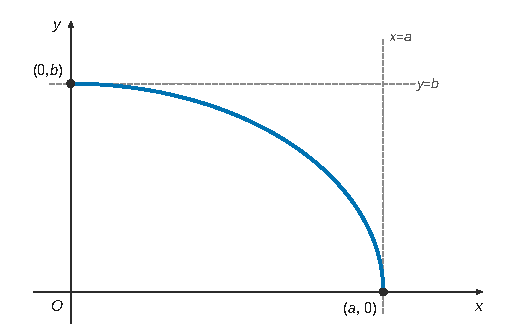
\includegraphics{figures/q7-courbe-cf.pdf}
\caption*{Figure 1 --- Tracé de 𝒞\_f (Q7) : tangente horizontale y = b en (0, b),
demi-tangente verticale x = a en (a, 0) ; tracé avec a = 3, b = 2}
\end{figure}

L'arc part horizontalement de \((0,b)\) et arrive verticalement en \((a,0)\).

D'après Q5, pour \(x\in[0,a]\), le point \((x,f(x))\) vérifie
\equationajustee{\frac{x^2}{a^2}+\frac{f(x)^2}{b^2}=1,}
avec \(f(x)\geqslant 0\). Donc \({\mathcal{C}}_f\) est exactement le quart de \(\mathcal{E}\) contenu dans \(\{x\geqslant 0,\ y\geqslant 0\}\).

\textbf{Q8.} L'équation de Q5 est invariante par \((x,y)\mapsto(-x,y)\) et par \((x,y)\mapsto(x,-y)\). Ainsi \(\mathcal{E}\) est symétrique par rapport aux deux axes.

De plus, soit \((x,y)\in\mathcal{E}\) avec \(x\geqslant0\) et \(y\geqslant0\). Alors \(x\in[0,a]\) et \(y=f(x)\).
Donc \(\mathcal{E}\) est la réunion de \({\mathcal{C}}_f\) et de ses images par les symétries par rapport aux deux axes et à l'origine.

\begin{figure}[H]
\centering
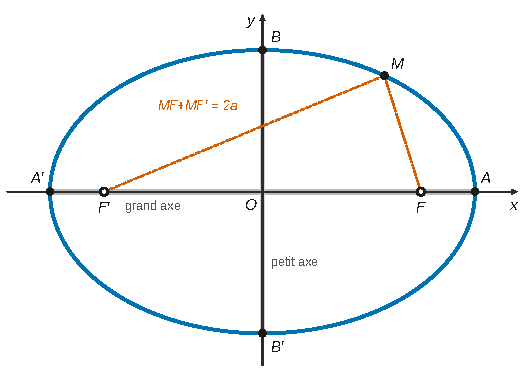
\includegraphics{figures/q8-ellipse-foyers.pdf}
\caption*{Figure 2 --- L'ellipse ℰ (Q8) : sommets A, A′, B, B′, foyers F, F′ sur
le grand axe, et un point M avec MF + MF′ = 2a ; tracé avec a = 3, b =
2, c = √5}
\end{figure}

Les tangentes sont verticales en \(A(a,0)\) et \(A'(-a,0)\). Elles sont horizontales en \(B(0,b)\) et \(B'(0,-b)\).
Comme \(b<a\), \(\mathcal{E}\) est allongée horizontalement. Puisque \(0<c<a\), les foyers \(F(c,0)\) et \(F'(-c,0)\) sont strictement entre le centre et les sommets.

\hypertarget{iii-paramuxe8tres-de-lellipse}{%
\subsection{III --- Paramètres de l'ellipse}\label{iii-paramuxe8tres-de-lellipse}}

\textbf{Q9.} De \(0<c<a\) et \(a>0\), on tire \(0<\frac ca<1\) :
\equationajustee{\boxed{e\in\,]0,1[.}}
Puis \(\boxed{c=ae}\). Comme \(a>0\) et \(1-e^2>0\),
\equationajustee{\boxed{\begin{aligned}
b&=\sqrt{a^2-a^2e^2}\\
&=a\sqrt{1-e^2}.
\end{aligned}}}

\textbf{Q10.} On raisonne à \(a\) fixé (le grand axe est fixé).

\emph{Si \(e\) est proche de \(0\).} Le demi-petit axe \(b=a\sqrt{1-e^2}\) est proche de \(a\), et \(c=ae\) est presque nul.
L'ellipse est presque le cercle de centre \(O\) et de rayon \(a\), et ses foyers sont proches du centre.

\emph{Si \(e\) est proche de \(1\).} Alors \(b\) est presque nul et \(c\) est proche de \(a\).
L'ellipse est très aplatie le long de son grand axe \([A'A]\), presque confondue avec ce segment, et ses foyers sont proches des sommets \(A\) et \(A'\).

\begin{center}\rule{0.5\linewidth}{0.5pt}\end{center}

\hypertarget{partie-b-uxe9tude-du-mouvement-des-planuxe8tes-massives-du-systuxe8me-solaire-sans-nuxe9gliger-les-interactions}{%
\section{Partie B --- Étude du mouvement des planètes massives du système solaire sans négliger les interactions}\label{partie-b-uxe9tude-du-mouvement-des-planuxe8tes-massives-du-systuxe8me-solaire-sans-nuxe9gliger-les-interactions}}

\textbf{Q11.} Écrivons \(B=(\beta_{ij})\), à coefficients constants. La relation \(G_t=BL_t\) s'écrit \(h_i'(t)=\sum_{j}\beta_{ij}l_j(t)\) pour \(i\in\llbracket1,3\rrbracket\).
Les \(l_j\) étant dérivables et les \(\beta_{ij}\) constants, on dérive :
\equationajustee{h_i''(t)=\sum_j\beta_{ij}l_j'(t),}
c'est-à-dire \(F_t=BK_t\). Avec \(K_t=-BH_t\), on obtient pour tout \(t\in{\mathbb{R}}_+\) :
\equationajustee{\boxed{\begin{aligned}
F_t&=B(-BH_t)\\
&=A\,H_t,\\
\text{avec}\quad A&=-B^2.
\end{aligned}}}

\textbf{Q12.} La matrice \(A\in{\mathcal{M}}_3(\mathbb{R})\) possède trois valeurs propres réelles deux à deux distinctes \(\lambda_1<\lambda_2<\lambda_3\). Une matrice de \({\mathcal{M}}_3(\mathbb{R})\) ayant trois valeurs propres réelles distinctes est diagonalisable dans \({\mathcal{M}}_3(\mathbb{R})\).

En effet, soit \(X_i\) un vecteur propre associé à \(\lambda_i\). La famille \((X_1,X_2,X_3)\) est libre (vecteurs propres associés à des valeurs propres distinctes), donc c'est une base de \({\mathbb{R}}^3\).
La matrice \(Q\) de colonnes \(X_1,X_2,X_3\) est inversible et vérifie \(AQ=Q\,\mathrm{diag}(\lambda_1,\lambda_2,\lambda_3)\), d'où
\equationajustee{\boxed{A=Q\begin{pmatrix}\lambda_1&0&0\\0&\lambda_2&0\\0&0&\lambda_3\end{pmatrix}Q^{-1},\qquad Q\in{\mathrm{GL}}_3(\mathbb{R}).}}

\textbf{Q13.} Notons \(\Delta=\mathrm{diag}(\lambda_1,\lambda_2,\lambda_3)\). Chaque \(y_i\) est combinaison linéaire à coefficients constants des \(h_j\), donc deux fois dérivable, et
\equationajustee{\begin{aligned}
Y_t''&=Q^{-1}H_t''\\
&=Q^{-1}F_t\\
&=Q^{-1}AH_t\\
&=Q^{-1}Q\Delta Q^{-1}H_t\\
&=\Delta Y_t.
\end{aligned}}
Ligne par ligne, pour tout \(i\in\llbracket1,3\rrbracket\) :
\equationajustee{\boxed{y_i''-\lambda_i\,y_i=0.}}
C'est une équation différentielle linéaire homogène d'ordre 2 à coefficients constants. Avec \(\omega_i=\sqrt{-\lambda_i}>0\), elle s'écrit \(y_i''+\omega_i^2y_i=0\).

\textbf{Q14.} L'équation caractéristique \(r^2-\lambda_i=0\) a pour racines \(\pm i\omega_i\), car \(\lambda_i<0\). Les solutions réelles sont donc les fonctions
\equationajustee{\boxed{y_i(t)=\alpha_i\cos\big(\sqrt{-\lambda_i}\,t\big)+\beta_i\sin\big(\sqrt{-\lambda_i}\,t\big),}}
où \((\alpha_i,\beta_i)\in{\mathbb{R}}^2\).
On peut aussi écrire \(y_i(t)=C_i\cos(\omega_it-\varphi_i)\), avec \(C_i\geqslant 0\) et \(\varphi_i\in\mathbb{R}\). C'est une oscillation de pulsation \(\sqrt{-\lambda_i}\).

\textbf{Q15.} \emph{Inversibilité de \(B\).} La matrice \(A\) est semblable à \(\Delta\), donc \(\det A=\lambda_1\lambda_2\lambda_3\neq0\). Or
\equationajustee{\begin{aligned}
\det A&=\det(-B^2)\\
&=(-1)^3\det(B)^2\\
&=-\det(B)^2.
\end{aligned}}
Donc \(\det B\neq0\) :
\equationajustee{\boxed{B\in{\mathrm{GL}}_3(\mathbb{R}).}}
\emph{Expression des \(h_i\).} De \(Y_t=Q^{-1}H_t\) :
\equationajustee{\boxed{\begin{aligned}
H_t&=Q\,Y_t,\\
\text{soit}\quad h_i(t)&=\sum_{j=1}^3 q_{ij}\,y_j(t),
\end{aligned}}}
où \(Q=(q_{ij})\).

\emph{Expression des \(l_i\).} Comme \(B\) est inversible, \(G_t=BL_t\) donne \(L_t=B^{-1}G_t\).
Or \(G_t=H_t'\), et \(H_t'=QY_t'\) car \(Q\) est constante. Donc
\equationajustee{\boxed{\begin{aligned}
L_t&=B^{-1}Q\,Y_t',\\
\text{soit}\quad l_i(t)&=\sum_{j=1}^3 r_{ij}\,y_j'(t),
\end{aligned}}}
où \(B^{-1}Q=(r_{ij})\), avec
\equationajustee{y_j'(t)=\omega_j\big(-\alpha_j\sin(\omega_jt)+\beta_j\cos(\omega_jt)\big).}

\begin{center}\rule{0.5\linewidth}{0.5pt}\end{center}

\hypertarget{partie-c-muxe9thode-de-le-verrier-pour-duxe9terminer-les-valeurs-propres}{%
\section{Partie C --- Méthode de Le Verrier pour déterminer les valeurs propres}\label{partie-c-muxe9thode-de-le-verrier-pour-duxe9terminer-les-valeurs-propres}}

\hypertarget{i-ruxe9solution-des-uxe9quations}{%
\subsection{I --- Résolution des équations}\label{i-ruxe9solution-des-uxe9quations}}

\textbf{Q16.} Pour \(A=(a_{ij})\), \(B=(b_{ij})\) dans \({\mathcal{M}}_3(\mathbb{R})\) :
\equationajustee{\begin{aligned}
\mathrm{Tr}(AB)&=\sum_{i=1}^3(AB)_{ii}\\
&=\sum_{i=1}^3\sum_{j=1}^3a_{ij}b_{ji}\\
&=\sum_{j=1}^3\sum_{i=1}^3b_{ji}a_{ij}\\
&=\sum_{j=1}^3(BA)_{jj}\\
&=\mathrm{Tr}(BA).
\end{aligned}}
Soit \(N=P^{-1}MP\) avec \(P\in{\mathrm{GL}}_3(\mathbb{R})\). Alors
\equationajustee{\begin{aligned}
\mathrm{Tr}(N)&=\mathrm{Tr}\big(P^{-1}(MP)\big)\\
&=\mathrm{Tr}\big((MP)P^{-1}\big)\\
&=\mathrm{Tr}(M).
\end{aligned}}
\textbf{Deux matrices semblables ont donc même trace.}

\textbf{Q17.} Notons \(\Delta=\mathrm{diag}(\lambda_1,\lambda_2,\lambda_3)\). Par récurrence, \(A^k=Q\Delta^kQ^{-1}\) pour \(k\in{\mathbb{N}}^*\). En effet, si c'est vrai au rang \(k\), alors
\equationajustee{\begin{aligned}
A^{k+1}&=Q\Delta^kQ^{-1}Q\Delta Q^{-1}\\
&=Q\Delta^{k+1}Q^{-1}.
\end{aligned}}
Donc \(A^k\) est semblable à \(\Delta^k=\mathrm{diag}(\lambda_1^k,\lambda_2^k,\lambda_3^k)\) et, par Q16,
\equationajustee{\boxed{\begin{aligned}
\mathrm{Tr}(A)&=S_1,\\
\mathrm{Tr}(A^2)&=S_2,\\
\mathrm{Tr}(A^3)&=S_3.
\end{aligned}}}

\textbf{Q18.} On a \(XI_3-A=Q(XI_3-\Delta)Q^{-1}\), donc
\equationajustee{\begin{aligned}
P_A&=\det(Q)\det(XI_3-\Delta)\det(Q^{-1})\\
&=\det(XI_3-\Delta).
\end{aligned}}
Ainsi
\equationajustee{\boxed{P_A=(X-\lambda_1)(X-\lambda_2)(X-\lambda_3).}}
En développant :
\equationajustee{P_A=X^3-(\lambda_1+\lambda_2+\lambda_3)X^2+(\lambda_1\lambda_2+\lambda_1\lambda_3+\lambda_2\lambda_3)X-\lambda_1\lambda_2\lambda_3.}
Par identification (\(\alpha_3=1\)) :
\equationajustee{\boxed{\begin{aligned}
\alpha_0&=-\lambda_1\lambda_2\lambda_3,\\
\alpha_1&=\lambda_1\lambda_2+\lambda_1\lambda_3+\lambda_2\lambda_3,\\
\alpha_2&=-(\lambda_1+\lambda_2+\lambda_3).
\end{aligned}}}

\textbf{Q19.} D'abord \(\alpha_2=-S_1\). Ensuite
\equationajustee{\begin{aligned}
S_1^2&=\lambda_1^2+\lambda_2^2+\lambda_3^2+2(\lambda_1\lambda_2+\lambda_1\lambda_3+\lambda_2\lambda_3)\\
&=S_2+2\alpha_1.
\end{aligned}}
Donc
\equationajustee{\boxed{\begin{aligned}
\alpha_2&=-S_1,\\
\alpha_1&=\frac{S_1^2-S_2}{2},
\end{aligned}}}
et, avec la valeur admise de \(\alpha_0\) et Q17,
\equationajustee{P_A=X^3-\mathrm{Tr}(A)X^2+\frac{\mathrm{Tr}(A)^2-\mathrm{Tr}(A^2)}{2}X+\frac{3\,\mathrm{Tr}(A)\mathrm{Tr}(A^2)-\mathrm{Tr}(A)^3-2\,\mathrm{Tr}(A^3)}{6}.}

\hypertarget{ii-uxe9tude-dun-cas-particulier}{%
\subsection{II --- Étude d'un cas particulier}\label{ii-uxe9tude-dun-cas-particulier}}

On pose \(N=2A\), de sorte que \(A^k=N^k/2^k\) :
\equationajustee{N=\begin{pmatrix}-4&11&13\\0&1&7\\0&7&1\end{pmatrix}.}

\textbf{Q20.} \(P_A\) est un polynôme de degré 3, scindé sur \(\mathbb{C}\) (théorème de d'Alembert-Gauss).
Toute matrice dont le polynôme caractéristique est scindé est trigonalisable. Il existe donc \(T\in{\mathcal{M}}_3(\mathbb{C})\) triangulaire supérieure et \(Q\in{\mathrm{GL}}_3(\mathbb{C})\) telles que
\equationajustee{\boxed{A=QTQ^{-1}.}}

Notons \(\mu_1,\mu_2,\mu_3\) les coefficients diagonaux de \(T\). Le calcul de Q16 vaut sur \(\mathbb{C}\).

Un produit de matrices triangulaires supérieures est triangulaire supérieure, de diagonale le produit des diagonales. Donc \(A^k=QT^kQ^{-1}\) donne
\equationajustee{\mathrm{Tr}(A^k)=\mu_1^k+\mu_2^k+\mu_3^k.}
De même, le déterminant d'une matrice triangulaire étant le produit de ses coefficients diagonaux,
\equationajustee{\begin{aligned}
P_A&=\det(XI_3-T)\\
&=(X-\mu_1)(X-\mu_2)(X-\mu_3).
\end{aligned}}
Les calculs de Q17 à Q19 se transposent mot pour mot : \textbf{oui, les relations de Q19 restent valables}, avec \(S_k=\mathrm{Tr}(A^k)\), somme des puissances \(k\)-ièmes des valeurs propres complexes comptées avec multiplicité.

\textbf{Q21.} Calcul direct :
\equationajustee{\begin{aligned}
N^2&=\begin{pmatrix}16&58&38\\0&50&14\\0&14&50\end{pmatrix},\\
N^3&=\begin{pmatrix}-64&500&652\\0&148&364\\0&364&148\end{pmatrix}.
\end{aligned}}
Donc \(\mathrm{Tr}(N)=-2\), \(\mathrm{Tr}(N^2)=116\) et \(\mathrm{Tr}(N^3)=232\).
Comme \(\mathrm{Tr}(A^k)=\mathrm{Tr}(N^k)/2^k\), on divise respectivement par 2, 4 et 8 :
\equationajustee{\boxed{\begin{aligned}
\mathrm{Tr}(A)&=-1,\\
\mathrm{Tr}(A^2)&=29,\\
\mathrm{Tr}(A^3)&=29.
\end{aligned}}}
Par Q19 et Q20, avec \(S_1=-1\), \(S_2=29\) et \(S_3=29\) :
\equationajustee{\begin{aligned}
\alpha_2&=1,\\
\alpha_1&=\frac{1-29}{2}\\
&=-14,\\
\alpha_0&=\frac{3(-1)(29)-(-1)-2\cdot29}{6}\\
&=\frac{-144}{6}\\
&=-24,
\end{aligned}}
et \(\alpha_3=1\), d'où
\equationajustee{\boxed{\begin{aligned}
P_A&=X^3+X^2-14X-24\\
&=R.
\end{aligned}}}

\textbf{Q22.} Les valeurs propres de \(A\) sont les racines de \(R\). On a
\equationajustee{\begin{aligned}
R(-2)&=-8+4+28-24\\
&=0,
\end{aligned}}
donc \(R=(X+2)(X^2-X-12)\). Le trinôme a pour discriminant \(49\) et pour racines \(4\) et \(-3\).
Donc \(R=(X+2)(X+3)(X-4)\) et
\equationajustee{\boxed{\mathrm{Sp}(A)=\{-3,\,-2,\,4\}.}}

\textbf{Q23.} On a \(AX=\lambda X\iff NX=2\lambda X\).

\emph{Pour \(\lambda=-2\).} Le système \((N+4I_3)X=0\) s'écrit
\equationajustee{\begin{aligned}
11y+13z&=0,\\
5y+7z&=0,\\
7y+5z&=0.
\end{aligned}}
Le système en \((y,z)\) formé des deux dernières équations a pour déterminant \(25-49\neq0\). Donc \(y=z=0\) et \(x\) est libre : \(X_1=(1,0,0)^\top\).

\emph{Pour \(\lambda=-3\).} Le système \((N+6I_3)X=0\) s'écrit
\equationajustee{\begin{aligned}
2x+11y+13z&=0,\\
7y+7z&=0.
\end{aligned}}
Donc \(y=-z\) et \(x=-z\) : \(X_2=(1,1,-1)^\top\).

\emph{Pour \(\lambda=4\).} Le système \((N-8I_3)X=0\) s'écrit
\equationajustee{\begin{aligned}
-12x+11y+13z&=0,\\
-7y+7z&=0.
\end{aligned}}
Donc \(y=z\) et \(x=2z\) : \(X_3=(2,1,1)^\top\).

Vérifications :
\equationajustee{\begin{aligned}
NX_1&=-4X_1,\\
NX_2&=(-6,-6,6)^\top\\
&=-6X_2,\\
NX_3&=(16,8,8)^\top\\
&=8X_3.
\end{aligned}}
Ces vecteurs propres sont associés à des valeurs propres distinctes : ils forment une base, et la matrice qu'ils forment a pour déterminant \(2\neq0\). Ainsi
\equationajustee{\boxed{\begin{aligned}
Q&=\begin{pmatrix}1&1&2\\0&1&1\\0&-1&1\end{pmatrix}\in{\mathrm{GL}}_3(\mathbb{R}),\\
Q^{-1}AQ&=\begin{pmatrix}-2&0&0\\0&-3&0\\0&0&4\end{pmatrix}.
\end{aligned}}}

\begin{center}\rule{0.5\linewidth}{0.5pt}\end{center}

\hypertarget{partie-d-perturbation-sur-une-matrice-dordre-3}{%
\section{Partie D --- Perturbation sur une matrice d'ordre 3}\label{partie-d-perturbation-sur-une-matrice-dordre-3}}

Rappel : \(a<b<c\) ; \(u,v,w\) sont non nuls, donc \(u^2,v^2,w^2>0\).
On a \(U=(u,v,w)^\top\), \(T=UU^\top\) et \(D=\mathrm{diag}(a,b,c)\). Enfin \(t\neq0\) et \(D(t)=D+tT\).
On note, sur \(\mathbb{R}\setminus\{a,b,c\}\),
\equationajustee{F(\lambda)=\frac{u^2}{\lambda-a}+\frac{v^2}{\lambda-b}+\frac{w^2}{\lambda-c}.}

\hypertarget{i-solutions-et-spectre}{%
\subsection{I --- Solutions et spectre}\label{i-solutions-et-spectre}}

\textbf{Q24.} La matrice \(\lambda I_3-D=\mathrm{diag}(\lambda-a,\lambda-b,\lambda-c)\) a ses coefficients diagonaux non nuls, puisque \(\lambda\notin\{a,b,c\}\). Donc \(\boxed{\lambda I_3-D\in{\mathrm{GL}}_3(\mathbb{R})}\), d'inverse
\equationajustee{(\lambda I_3-D)^{-1}=\mathrm{diag}\Big(\frac1{\lambda-a},\frac1{\lambda-b},\frac1{\lambda-c}\Big).}

Soit \(X\neq0\) avec \(D(t)X=\lambda X\). Alors \(DX+tU(U^\top X)=\lambda X\), donc
\equationajustee{\begin{aligned}
(\lambda I_3-D)X&=tU(U^\top X),\\
X&=t(\lambda I_3-D)^{-1}U(U^\top X).
\end{aligned}}
En multipliant à gauche par \(U^\top\) :
\equationajustee{\boxed{U^\top X=t\,U^\top(\lambda I_3-D)^{-1}UU^\top X.}}

\textbf{Q25.} Posons \(s=U^\top X\in\mathbb{R}\). Si \(s=0\), la relation \(X=t(\lambda I_3-D)^{-1}U\,s\) donne \(X=0\), ce qui est exclu.
Donc \(s\neq0\). En simplifiant Q24 par \(s\), on obtient \(t\,U^\top(\lambda I_3-D)^{-1}U=1\).
Comme \(t\neq0\),
\equationajustee{\boxed{U^\top(\lambda I_3-D)^{-1}U=\frac1t.}}

\textbf{Q26.} Par Q24,
\equationajustee{(\lambda I_3-D)^{-1}U=\Big(\frac{u}{\lambda-a},\frac{v}{\lambda-b},\frac{w}{\lambda-c}\Big)^\top,}
donc \(U^\top(\lambda I_3-D)^{-1}U=F(\lambda)\). Par Q25,
\equationajustee{\boxed{F(\lambda)=\frac1t.}}
\textbf{Ainsi \(\lambda\) est solution de \((E_t)\).}

\textbf{Q27.} \(F\) est dérivable sur \(\mathbb{R}\setminus\{a,b,c\}=I_1\cup I_2\cup I_3\cup I_4\), avec
\equationajustee{\begin{aligned}
I_1&=\,]-\infty,a[,\\
I_2&=\,]a,b[,\\
I_3&=\,]b,c[,\\
I_4&=\,]c,+\infty[.
\end{aligned}}
Sur chacun d'eux,
\equationajustee{F'(\lambda)=-\frac{u^2}{(\lambda-a)^2}-\frac{v^2}{(\lambda-b)^2}-\frac{w^2}{(\lambda-c)^2}<0.}
\(F\) est donc strictement décroissante sur chacun des quatre intervalles.

\emph{Limites.} Chaque terme tend vers \(0\) en \(\pm\infty\). Au voisinage de \(a\), les deux autres termes ont une limite finie, et
\equationajustee{\lim_{\lambda\to a^{\mp}}\frac{u^2}{\lambda-a}=\mp\infty.}
Il en va de même en \(b\) et en \(c\).
Sur \(I_1\), les trois termes sont négatifs, donc \(F<0\). Sur \(I_4\), ils sont positifs, donc \(F>0\).

\begin{longtable}[]{@{}
  >{\raggedright\arraybackslash}p{(\columnwidth - 18\tabcolsep) * \real{0.1165}}
  >{\raggedright\arraybackslash}p{(\columnwidth - 18\tabcolsep) * \real{0.0930}}
  >{\raggedright\arraybackslash}p{(\columnwidth - 18\tabcolsep) * \real{0.1361}}
  >{\raggedright\arraybackslash}p{(\columnwidth - 18\tabcolsep) * \real{0.0609}}
  >{\raggedright\arraybackslash}p{(\columnwidth - 18\tabcolsep) * \real{0.1111}}
  >{\raggedright\arraybackslash}p{(\columnwidth - 18\tabcolsep) * \real{0.0609}}
  >{\raggedright\arraybackslash}p{(\columnwidth - 18\tabcolsep) * \real{0.1111}}
  >{\raggedright\arraybackslash}p{(\columnwidth - 18\tabcolsep) * \real{0.0609}}
  >{\raggedright\arraybackslash}p{(\columnwidth - 18\tabcolsep) * \real{0.1267}}
  >{\raggedright\arraybackslash}p{(\columnwidth - 18\tabcolsep) * \real{0.0930}}@{}}
\toprule\noalign{}
\begin{minipage}[b]{\linewidth}\raggedright
\(\lambda\)
\end{minipage} & \begin{minipage}[b]{\linewidth}\raggedright
\(-\infty\)
\end{minipage} & \begin{minipage}[b]{\linewidth}\raggedright
\end{minipage} & \begin{minipage}[b]{\linewidth}\raggedright
\(a\)
\end{minipage} & \begin{minipage}[b]{\linewidth}\raggedright
\end{minipage} & \begin{minipage}[b]{\linewidth}\raggedright
\(b\)
\end{minipage} & \begin{minipage}[b]{\linewidth}\raggedright
\end{minipage} & \begin{minipage}[b]{\linewidth}\raggedright
\(c\)
\end{minipage} & \begin{minipage}[b]{\linewidth}\raggedright
\end{minipage} & \begin{minipage}[b]{\linewidth}\raggedright
\(+\infty\)
\end{minipage} \\
\midrule\noalign{}
\endhead
\bottomrule\noalign{}
\endlastfoot
\(F'(\lambda)\) & & \(-\) & ‖ & \(-\) & ‖ & \(-\) & ‖ & \(-\) & \\
\(F\) & 0⁻ & décroît vers −∞ & ‖ & de +∞ à −∞ & ‖ & de +∞ à −∞ & ‖ & décroît de +∞ & 0⁺ \\
\end{longtable}

Par le théorème de la bijection (continuité et stricte monotonie sur un intervalle), \(F\) réalise des bijections
\equationajustee{\begin{aligned}
I_1&\to\,]-\infty,0[,\\
I_2&\to\mathbb{R},\\
I_3&\to\mathbb{R},\\
I_4&\to\,]0,+\infty[.
\end{aligned}}
Ainsi \(F\) ne s'annule ni sur \(I_1\) ni sur \(I_4\).
Elle s'annule exactement une fois sur \(I_2\) et une fois sur \(I_3\) :
\equationajustee{\boxed{\begin{aligned}{}&F \text{ s'annule exactement en } \rho_1\in\,]a,b[ \text{ et } \rho_2\in\,]b,c[,\\
&a<\rho_1<b<\rho_2<c.
\end{aligned}}}

\textbf{Q28.} L'équation \((E_t)\) s'écrit \(F(\lambda)=\frac1t\). On utilise les bijections de Q27 et la décroissance de \(F\), avec \(F(\rho_i)=0\).

\begin{figure}[H]
\centering
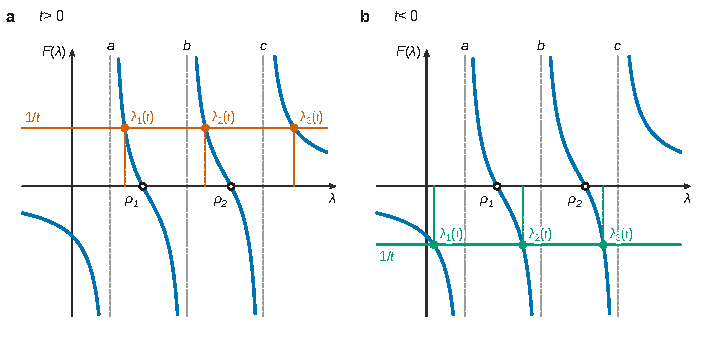
\includegraphics{figures/q28-graphe-f-droite-1-sur-t.pdf}
\caption*{Figure 3 --- Résolution graphique de (Eₜ) (Q28) : la droite d'ordonnée
1/t coupe le graphe de F en λ₁(t) \textless{} λ₂(t) \textless{} λ₃(t),
(a) pour t \textgreater{} 0, (b) pour t \textless{} 0 ; tracé avec a =
1, b = 3, c = 5, u² = v² = w² = 1}
\end{figure}

\emph{Cas \(t>0\)}, donc \(\frac1t>0\). Il n'y a aucune solution dans \(I_1\).
Il y a une unique solution dans \(I_2\), et \(F(\lambda)=\frac1t>0=F(\rho_1)\) impose \(\lambda<\rho_1\).
De même, il y a une unique solution dans \(I_3\), inférieure à \(\rho_2\), et une unique solution dans \(I_4\). D'où
\equationajustee{\boxed{t>0:\quad a<\lambda_1(t)<\rho_1<b<\lambda_2(t)<\rho_2<c<\lambda_3(t).}}

\emph{Cas \(t<0\)}, donc \(\frac1t<0\). Il y a une unique solution dans \(I_1\).
Il y a une unique solution dans \(I_2\), supérieure à \(\rho_1\).
Il y en a une unique dans \(I_3\), supérieure à \(\rho_2\), et aucune dans \(I_4\). D'où
\equationajustee{\boxed{t<0:\quad \lambda_1(t)<a<\rho_1<\lambda_2(t)<b<\rho_2<\lambda_3(t)<c.}}
Dans les deux cas, \((E_t)\) a exactement trois solutions réelles, distinctes car situées dans des intervalles disjoints.

\textbf{Q29.} Notons \(\mathcal{S}\) l'ensemble des solutions de \((E_t)\).

\emph{\(a,b,c\) ne sont pas valeurs propres de \(D(t)\).} Supposons \(D(t)X=aX\).
Alors \((aI_3-D)X=tU(U^\top X)\), avec \(aI_3-D=\mathrm{diag}(0,a-b,a-c)\).
La première ligne de \(aI_3-D\) est nulle, donc \(tu\,(U^\top X)=0\). Comme \(t\) et \(u\) sont non nuls, \(U^\top X=0\).
Alors \(\mathrm{diag}(0,a-b,a-c)X=0\) donne \(x_2=x_3=0\).
Puis \(U^\top X=ux_1=0\) donne \(x_1=0\), donc \(X=0\).
Le même raisonnement vaut pour \(b\), avec \(v\neq0\). Il vaut aussi pour \(c\), avec \(w\neq0\).

\emph{\(\mathrm{Sp}(D(t))\subset\mathcal{S}\)} : une valeur propre de \(D(t)\) est donc dans \(\mathbb{R}\setminus\{a,b,c\}\), et Q24--Q26 s'appliquent.

\emph{\(\mathcal{S}\subset\mathrm{Sp}(D(t))\)} : soit \(\lambda\in\mathcal{S}\), donc \(\lambda\notin\{a,b,c\}\).
Posons \(X=(\lambda I_3-D)^{-1}U\) ; ce vecteur est non nul, car sa première composante \(\frac{u}{\lambda-a}\) est non nulle.
Alors \(DX=\lambda X-U\) et \(U^\top X=F(\lambda)=\frac1t\), donc
\equationajustee{\begin{aligned}
D(t)X&=DX+tU(U^\top X)\\
&=\lambda X-U+U\\
&=\lambda X.
\end{aligned}}
Ainsi \(\lambda\) est valeur propre de \(D(t)\). Par double inclusion,
\equationajustee{\boxed{\begin{aligned}
\mathcal{S}&=\mathrm{Sp}\big(D(t)\big)\\
&=\{\lambda_1(t),\lambda_2(t),\lambda_3(t)\}.
\end{aligned}}}

\hypertarget{ii-les-limites}{%
\subsection{II --- Les limites}\label{ii-les-limites}}

\textbf{Q30.} Pour chaque \(i\), la restriction de \(F\) à l'intervalle \(I_i\) est continue et strictement décroissante (Q27).
Par le théorème de la bijection, elle réalise une bijection de \(I_i\) sur \(F(I_i)\), dont la réciproque \(g_i\) est continue et strictement décroissante :
\equationajustee{\begin{aligned}
g_1&:\,]-\infty,0[\,\to\,]-\infty,a[,\\
g_2&:\mathbb{R}\to\,]a,b[,\\
g_3&:\mathbb{R}\to\,]b,c[,\\
g_4&:\,]0,+\infty[\,\to\,]c,+\infty[.
\end{aligned}}
Comme \(\rho_1\in\,]a,b[\) et \(F(\rho_1)=0\) : \(\boxed{g_2(0)=\rho_1}\).

La fonction \(g_2\) est décroissante et minorée par \(a\). Elle admet donc en \(+\infty\) une limite \(\ell\in[a,b[\).
Supposons \(\ell>a\) ; alors \(\ell\in I_2\). Par continuité de \(F\) en \(\ell\), on aurait
\equationajustee{y=F\big(g_2(y)\big)\xrightarrow[y\to+\infty]{}F(\ell),}
limite finie : c'est absurde. Donc \(\ell=a\).

De même, \(g_2\) est majorée par \(b\). Elle admet en \(-\infty\) une limite \(\ell'\in\,]a,b]\), et \(\ell'<b\) conduirait à la même contradiction. Ainsi
\equationajustee{\boxed{\begin{aligned}
\lim_{+\infty}g_2&=a,\\
\lim_{-\infty}g_2&=b.
\end{aligned}}}

\textbf{Q31.} Soit \(\lambda\in I_i\). D'après Q27 et Q28, il est solution de \((E_t)\) si et seulement si \(\frac1t\in F(I_i)\) et \(\lambda=g_i\big(\frac1t\big)\). Donc
\equationajustee{\boxed{\begin{aligned}
\text{pour } t>0:\quad\lambda_1(t)&=g_2\Big(\frac1t\Big),\\
\lambda_2(t)&=g_3\Big(\frac1t\Big),\\
\lambda_3(t)&=g_4\Big(\frac1t\Big);
\end{aligned}}}
\equationajustee{\boxed{\begin{aligned}
\text{pour } t<0:\quad\lambda_1(t)&=g_1\Big(\frac1t\Big),\\
\lambda_2(t)&=g_2\Big(\frac1t\Big),\\
\lambda_3(t)&=g_3\Big(\frac1t\Big).
\end{aligned}}}
Les domaines sont respectés. Pour \(t>0\), \(\frac1t\in\,]0,+\infty[\), domaine de \(g_4\).
Pour \(t<0\), \(\frac1t\in\,]-\infty,0[\), domaine de \(g_1\).

\textbf{Q32.} Par Q31,
\equationajustee{\begin{aligned}
\lambda_1&=g_2\circ\Big(t\mapsto\frac1t\Big)\quad\text{sur }]0,+\infty[,\\
\lambda_1&=g_1\circ\Big(t\mapsto\frac1t\Big)\quad\text{sur }]-\infty,0[.
\end{aligned}}
Par composition, \(\lambda_1\) est continue sur \({\mathbb{R}}^*\).

En \(0^+\) : \(\frac1t\to+\infty\) et, par Q30, \(\lambda_1(t)\to a\).

En \(0^-\) : \(\frac1t\to-\infty\). La fonction \(g_1\) est décroissante et majorée par \(a\).
Elle admet donc en \(-\infty\) une limite finie \(\ell\leqslant a\). Si l'on avait \(\ell<a\), la continuité de \(F\) en \(\ell\) donnerait
\equationajustee{y=F\big(g_1(y)\big)\xrightarrow[y\to-\infty]{}F(\ell),}
limite finie : c'est absurde. Donc \(g_1(y)\to a\) quand \(y\to-\infty\), et \(\lambda_1(t)\to a\).

Les deux limites coïncident : en posant \(\boxed{\lambda_1(0)=a}\), \(\lambda_1\) se prolonge en une fonction continue sur \(\mathbb{R}\). (Le même argument donne \(\lambda_2(0)=b\) et \(\lambda_3(0)=c\).)

\textbf{Q33.} \emph{Sur \({\mathbb{R}}^*\).} La fonction \(F\) est dérivable sur chaque \(I_i\) et \(F'\) ne s'y annule pas. Donc chaque \(g_i\) est dérivable (dérivée d'une bijection réciproque).
Par composition avec \(t\mapsto\frac1t\), la fonction \(\lambda_1\) est dérivable sur \({\mathbb{R}}^*\).

\emph{En \(0\).} Pour \(t\neq0\), on a \(\varepsilon(t)=\lambda_1(t)-a\neq0\) (Q28), et \(\varepsilon(t)\to0\) (Q32).
La relation \(F(\lambda_1(t))=\frac1t\), multipliée par \(t\), donne
\equationajustee{\frac{t\,u^2}{\varepsilon(t)}+t\left(\frac{v^2}{\lambda_1(t)-b}+\frac{w^2}{\lambda_1(t)-c}\right)=1.}
Comme \(\lambda_1(t)\to a\), avec \(a\neq b\) et \(a\neq c\), la parenthèse tend vers
\equationajustee{\frac{v^2}{a-b}+\frac{w^2}{a-c},}
qui est fini ; le second terme tend donc vers \(0\). Ainsi \(\frac{tu^2}{\varepsilon(t)}\to1\) et, comme \(u^2\neq0\),
\equationajustee{\begin{aligned}
\frac{\lambda_1(t)-\lambda_1(0)}{t}&=\frac{\varepsilon(t)}{t}\\
&\xrightarrow[t\to0]{}u^2.
\end{aligned}}
\(\lambda_1\) est donc dérivable en \(0\), donc sur \(\mathbb{R}\), et
\equationajustee{\boxed{\lambda_1'(0)=u^2.}}
En reprenant ce raisonnement :
\equationajustee{\boxed{\begin{aligned}
\lambda_2'(0)&=v^2,\\
\lambda_3'(0)&=w^2.
\end{aligned}}}

\textbf{Q34.} Pour \(t>0\), \(\lambda_1(t)=g_2(\frac1t)\). Quand \(t\to+\infty\), on a \(\frac1t\to0\).
Comme \(g_2\) est continue en \(0\), \(\lambda_1(t)\to g_2(0)=\rho_1\).

Pour \(t<0\), \(\lambda_1(t)=g_1(\frac1t)\). Quand \(t\to-\infty\), on a \(\frac1t\to0^-\).
La fonction \(g_1\) est décroissante sur \(]-\infty,0[\). Si elle était minorée au voisinage de \(0^-\), elle aurait une limite finie \(m<a\) en \(0^-\).
La continuité de \(F\) en \(m\) donnerait alors
\equationajustee{y=F\big(g_1(y)\big)\xrightarrow[y\to0^-]{}F(m),}
avec \(F(m)<0\) : c'est absurde. Donc \(g_1(y)\to-\infty\) quand \(y\to0^-\), et
\equationajustee{\boxed{\begin{aligned}
\lim_{t\to+\infty}\lambda_1(t)&=\rho_1,\\
\lim_{t\to-\infty}\lambda_1(t)&=-\infty.
\end{aligned}}}

\begin{figure}[H]
\centering
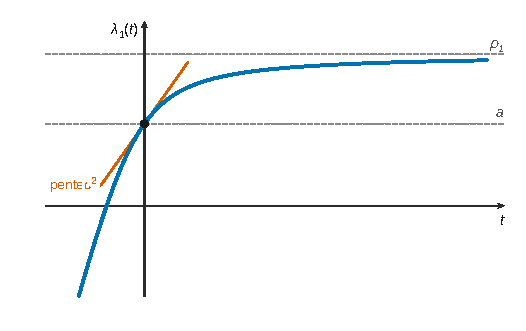
\includegraphics{figures/q34-allure-lambda1.pdf}
\caption*{Figure 4 --- Allure de λ₁ prolongée (Q32--Q34) : égale à a en 0 avec la
pente u², tendant vers ρ₁ en +∞ et vers −∞ en −∞ ; courbe calculée avec
a = 1, b = 3, c = 5, u² = v² = w² = 1}
\end{figure}

\emph{Commentaires.}

\textbf{Continuité du spectre.} On a \(\lambda_1(0)=a\), \(\lambda_2(0)=b\) et \(\lambda_3(0)=c\). Une petite perturbation \(tT\) de \(D\) ne déplace que peu ses valeurs propres.

\textbf{Sensibilité au premier ordre.} L'écart est proportionnel à \(t\), avec un coefficient explicite :
\equationajustee{\begin{aligned}
\lambda_1(t)&=a+u^2t+o(t),\\
\lambda_2(t)&=b+v^2t+o(t),\\
\lambda_3(t)&=c+w^2t+o(t).
\end{aligned}}
Contrôle : la somme des dérivées en \(0\), soit \(u^2+v^2+w^2\), est bien la dérivée de
\equationajustee{\mathrm{Tr}\,D(t)=a+b+c+t(u^2+v^2+w^2).}

\textbf{Sens et entrelacement.} Pour \(t>0\), chaque valeur propre est au-dessus de la valeur propre correspondante de \(D\) :
\equationajustee{a<\lambda_1(t)<b<\lambda_2(t)<c<\lambda_3(t).}
Elle est au-dessous pour \(t<0\). Les valeurs propres de \(D(t)\) et de \(D\) s'entrelacent.

\textbf{Comportement pour une grande perturbation.} Pour \(t\to+\infty\), \(\lambda_1(t)\to\rho_1\) et \(\lambda_2(t)=g_3(\frac1t)\to\rho_2\) restent bornées. Seule \(\lambda_3\) tend vers \(+\infty\).
Pour \(t\to-\infty\), \(\lambda_2\to\rho_1\) et \(\lambda_3\to\rho_2\). Seule \(\lambda_1\) tend vers \(-\infty\).
Une perturbation de rang 1 n'envoie à l'infini qu'une seule valeur propre.

\end{document}
